%#! platex thesis.tex

%======================================================================
% 章見出し
\chapter{文字認識に関する関連技術}
\label{cha:relate}
本章では,手書き文字認識技術として一般に用いられるオンライン文字認識とオフライン文字認識について説明する.さらに時系列データに対応した機械学習モデルである,再帰型ニューラルネットワークについて説明する.その後再帰型ニューラルネットワークを用いたオンライン文字認識の既存研究を述べ.遠隔医療での処方箋予測に向けたオンライン文字認識におけるデータ拡張に関する先行研究について述べる.
%----------------------------------------------------------------------

\section{手書き文字認識の種類}
\label{sec:rel_1}
手書き文字の認識は大きく2つに分けることができる.オフライン文字認識とオンライン文字認識である.オフライン文字認識は,文字の画像データにおいてそれぞれのピクセルが持つ情報を特徴量として文字を認識する技術であり,手書き文字は認識されるためにイメージスキャナやデジタルカメラによって読みとられる.
オンライン文字認識は手書き文字の$(x, y)$座標やスピード,筆圧などを特徴量として認識する技術で,通常タブレットなどに書き込まれた文字が認識される.

オフライン文字認識は画像認識技術であるため,文献\cite{yuan12:offline}のような畳み込みニューラルネットワーク(Convolutional Neural Network, 以下CNN)を用いた文字認識が多く研究されている.利用可能な画像データもインターネット上に多く存在するが,実際に認識を行う際には手書きされた文字をスキャナやデジタルカメラなどで読み取る必要があるなどのデメリットもある.

一方でオンライン文字認識はIAM On-Line Handwriting Database\cite{iam},CASIA Chinese Handwriting Database\cite{liu11:casia}などのデータセットが存在するが,オフライン文字認識に比べると利用可能なデータは少ない.しかし認識時においてはタブレットなどのデバイスに書き込まれた手書き文字のデータが直接使われるため,オフライン文字認識と比べると手間が少ない.また,オンライン文字認識は筆順・筆圧・書き込みにかかる時間などの,オフライン文字認識では使うことができない情報を用いて認識を行うことができるなどのメリットがある.

本研究では,医者の手書き文字は筆記体が多く使われるため画像での認識は難しいと考えられること,実際に使用する際にはスキャンやデジタルカメラによる撮影を行わずリアルタイムでの認識を想定していることから,オンライン文字認識を用いて医者の手書き医療用語の認識を行う.

%----------------------------------------------------------------------
\section{再帰型ニューラルネットワーク}
再帰型ニューラルネットワーク(Recurrent Neural Network,以下RNN)とは中間層に戻り値のある,音声,動画,文章などの時系列データの扱いに優れているニューラルネットワークである.以下でRNNの構造と,再帰型ニューラルネットワークの一種であるLong Short-Term Memory(以下,LSTM)について説明する.本論文ではLSTMを用いて機械学習を行う.
\subsection{RNNの構造}
\label{ssec:rel_2}

\begin{figure}[tb]
 \begin{center}
  \resizebox{\columnwidth}{!}{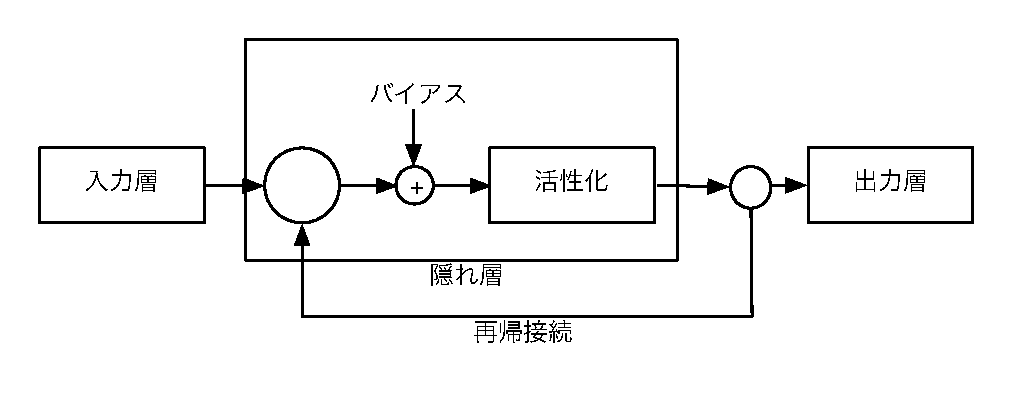
\includegraphics{img/rnn.eps}}
  \caption{RNNの構造}
  \label{rnn}
\end{center}
\end{figure}

\textbf{図~\ref{rnn}}に再帰型ニューラルネットワークの構造を示す.RNNは中間層のノードごとに戻り値があるため,現在入力されているデータより前のデータの影響を考慮して計算を行うことができる.そのためRNNは連続的な情報を保持したまま学習を行うことができる\cite{chakra16:bangla}.
式~\ref{eq:rnn-1}, 式~\ref{eq:rnn-2}に,RNNがそれぞれのノードにおいて行っている計算を入力値$x$と時間的順序$t$を用いて示す.
\begin{equation}
 H(t) = h(W_Hx(t) + W_{self}H(t-1) + b_H)
  \label{eq:rnn-1}
\end{equation}
\begin{equation}
 Y(t) = y(W_YH(t) + b_Y)
  \label{eq:rnn-2}
\end{equation}
ここにおいて$H(t)$は隠れ層の出力であり,$W_H$は隠れ層への入力の重み,$W_{self}$は戻り値の重み,$b_H$は隠れ層へのバイアス,$Y(t)$はネットワークの出力,$W_Y$は隠れ層の出力の重み,$b_Y$は出力へのバイアス,$y()$と$h()$はそれぞれ出力層と隠れ層の活性化関数である.式より,隠れ層の出力は隠れ層への入力$x(t)$だけでなく,隠れ層からの1つ前の出力$H(t-1)$の影響も受けていることがわかる.したがってネットワークの出力$Y(t)$は$x(t)$と$x(t-1)$の影響を受けていると言える.この計算は最初をのぞいた全ての入力において行われている.

\begin{figure}[tb]
 \begin{center}
  \resizebox{\columnwidth}{!}{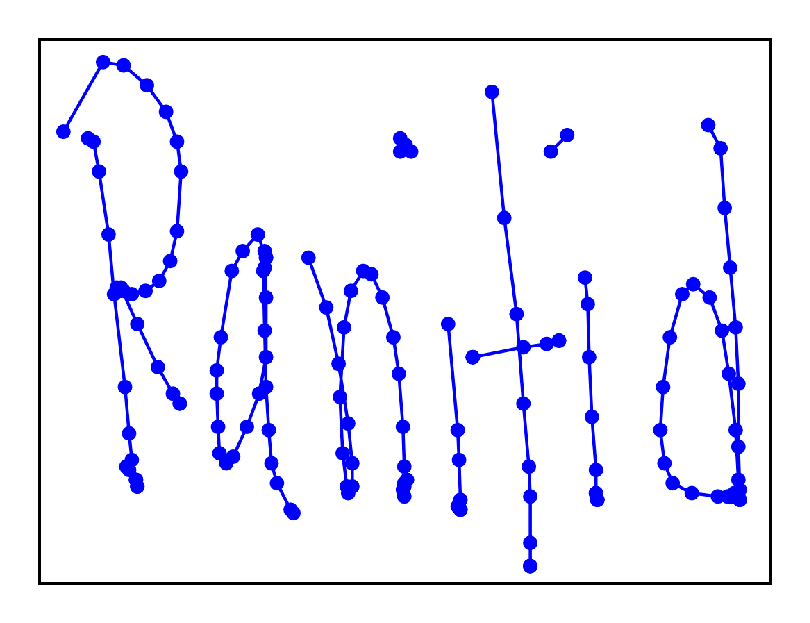
\includegraphics{img/ranitid.eps}}
  \caption{文字を点で表した図}
  \label{original}
\end{center}
\end{figure}

\textbf{図~\ref{original}}に認識する手書き文字の例を示す.このように,手書き文字は検出された座標が時間的順序に従って並んだものであると言える.オフライン文字認識では,手書き文字を画像データとして捉えるため,点の時間的順序を考慮に入れずに認識を行う.RNNの入力に連続した手書き文字の点データを用いることで,オンライン文字認識ではその時間的順序を考慮に入れて認識を行うことができる.

しかし,実際にRNNで出力に反映できる過去の入力情報は短く,時系列10ステップ分程度であると言われている\cite{okatani15:deep_learning}.

\subsection{LSTM}
\label{ssec:lstm}

\begin{figure}[tb]
 \begin{center}
  \resizebox{\columnwidth}{!}{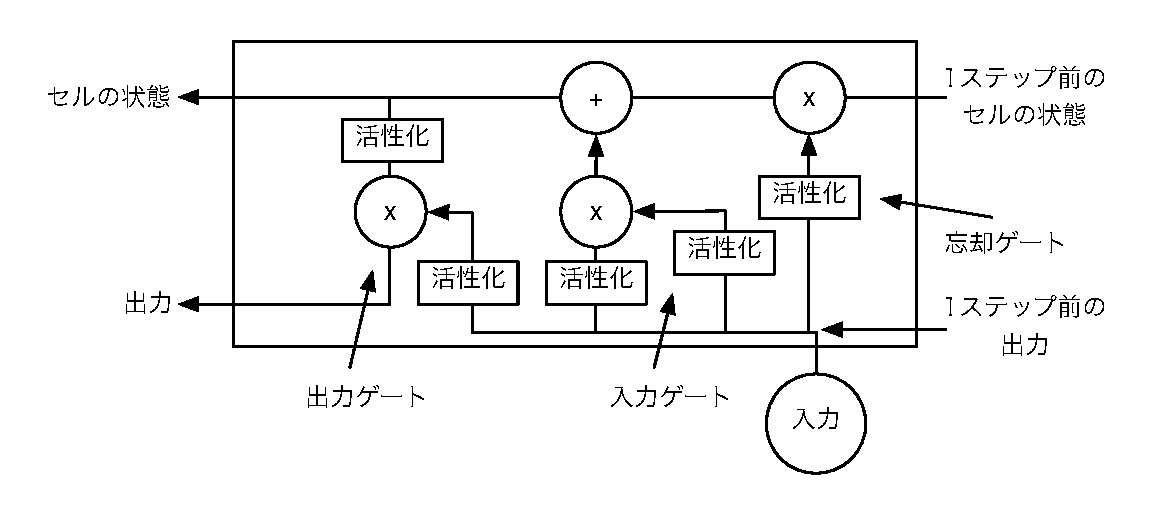
\includegraphics{img/lstm.eps}}
  \caption{LSTMブロックの構造}
  \label{lstm}
\end{center}
\end{figure}

\textbf{図~\ref{lstm}}にLSTMブロックの構造を示す.LSTMはRNNよりも長期にわたる記憶を実現するための方法のひとつで,RNNの隠れ層の各ユニットをLSTMブロックに置き換えたものである.RNNのユニットと異なり,LSTMブロックは記憶を持ったセルの構造をしている.ゲートと呼ばれる特殊な構造がセルに情報を与えるかセルの情報を除去するかを決める.

忘却ゲートがセル内の情報をリセットし,入力ゲートは,入力が現在のセルにどれだけ影響を与えるか決める.出力ゲートは出力が残りのネットワークにどれだけの影響を与えるか決める.この方法によってLSTMはより長い時系列データにおける再帰型ニューラルネットワークの利用を可能にしている.

%----------------------------------------------------------------------
\section{関連研究}
\label{sec:rel_3}
ここではLSTMを用いたオンライン文字認識の既存研究と,文字認識におけるデータ拡張に関する既存研究について述べる.

\subsection{直線データとBidirectionalLSTMを用いた中国語認識システム\cite{zhang18:drawing}}
\label{ssec:drawing}
文献\cite{zhang18:drawing}では中国語手書き漢字の座標データの中から,直線上の点や近接する点など,取り除いても文字として成り立つ点を除去したのち直線データに変換し,BidirectionalLSTMを用いて認識を行っている.BidirectionalLSTMについては\ref{sec:m_learning}節で述べる.点の除去を行うことで入力データを簡易化し,さらに直線データへの変更を行うことで連続する点同士の関係性(点同士の距離,次の点への角度,同一字画上にあるかなど)を特徴量として抽出することができる.機械学習モデルにはBidirectionalLSTMを用いることで,入力されているより過去の座標の情報だけでなく未来の座標の情報も考慮に入れた学習を行うことができる.

\subsection{dropStroke手法を用いたデータ拡張と筆者同定システム\cite{yang15:dropstroke}}
文献\cite{yang15:dropstroke}では中国語手書き漢字において,座標の時系列データから一部のストロークを除去する処理を複数回繰り返すことでデータ拡張を行い, CNN を用いたオフライン認識で筆者の同定を行っている.文字としては不完全なデータになるが筆者の特徴を大きく変えることにはならず,100\% に近い精度での筆者同定を可能にしている.ただし,ストロークを除去することで異なる文字・単語になってしまう可能性があり,本論文の目的とする単語認識においてこの手法は適切であるとは言えない.同著者からは,筆者同定のためのデータ拡張として dropSegment 手法というものも提案されているが\cite{yang16:dropsegment},これも異なる文字・単語に変わってしまう可能性があり,単語認識に適切であるとは言えない.

%================================================================================================
\section{先行研究}
\label{sec:rel_4}
遠隔医療システムにおける処方箋予測に向けた手書き医療用語認識に関する研究\cite{takahashi}では,処方箋の予測に向けたシステムの初期研究として,再帰型ニューラルネットワークの一種であるBidirectionalLSTMを用いたオンライン手書き医療用語認識手法の提案を行っている.また様々な手書き文字に対応するため,文字認識では多様な提供者から大量のデータを得る必要がある.しかし,十分なデータ量を確保するためには非常に多くの労力と時間を要する.そこで筆者はオンライン手書き文字のデータ拡張手法として,ストロークの回転と平行移動によってデータ量を水増しするStroke Rotation and Parallel-shift(SRP)手法を提案している.
手書き文字データは,文献\cite{zhang18:drawing}を用いてデータの簡易化,特徴量の抽出を行っている.また文献\cite{takahashi}ではPortable Health Clinicにおける過去の処方箋データから頻出する単語を座標の時系列データとして収集している.収集した15991語のデータを用いて,SRP手法でデータ拡張を行った後にBidirectionalLSTMで学習を行った結果,480語のクラスにおいて89.5\%の精度で単語を認識している.この結果はデータ拡張を行わなかった場合の認識精度と比べて16.1\%高い.
しかしSRP手法において回転の大きさ,平行移動の大きさは筆者が文字の形を崩さないと判断できる範囲で設定しているため,データを高倍率で拡張した場合に同じような値を用いてしまい,拡張後に同じようなデータが増えて学習精度が低くなる原因になってしまう.そのため,この用語認識は学習の際にランダムに設定された回転の大きさと平行移動の大きさの組み合わせにより,認識精度にばらつきが出てしまうという問題がある.

先行研究\cite{takahashi}のBidirectionalLSTMを用いたオンライン手書き医療用語認識を説明する.また,オンライン文字認識用のデータ拡張手法として先行研究のSRP手法を説明する.

\subsection{システムの概要}
\label{sec:concept}
\textbf{図~\ref{sys_concept}} にシステムの概要を示す.提案システムでは,タブレットから収集した手書き医療用語の座標データに対して前処理を行う.その後学習プロセスでは前処理後のデータに拡張手法を適用し,機械学習における学習データとする.推定プロセスでは,学習を行ったモデルに前処理後のデータを入力し,用語を推定する.ニューラルネットワーク構造とデータ前処理,特徴量抽出に関しては\ref{ssec:drawing}項の文献\cite{takahashi}を参考にした.以下,各手順について述べる.

\begin{figure}[tb]
 \begin{center}
  \resizebox{\columnwidth}{!}{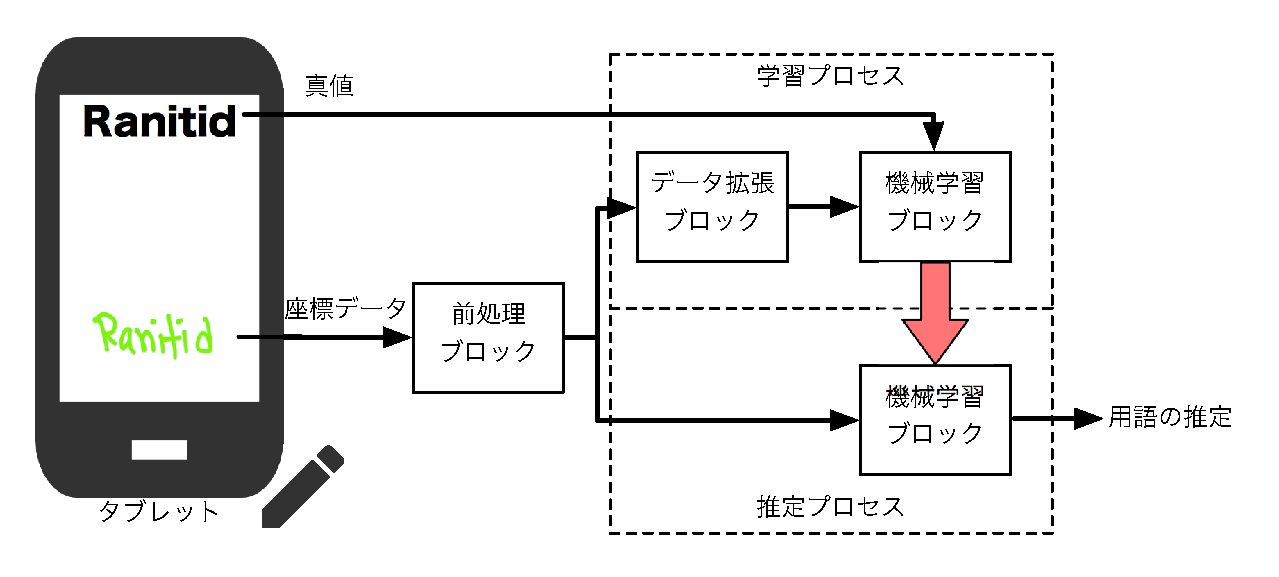
\includegraphics{img/system_structure.eps}}
  \caption{提案システムの概要}
  \label{sys_concept}
\end{center}
\end{figure}

\subsection{前処理ブロック}
\label{preprocess}
\textbf{図~\ref{preprocess}} に前処理ブロックの概要を示す.前処理ブロックでは,点の除去,正規化,特徴量抽出を行う.直線上の点や近接する点といった,取り除いても文字として成り立つような点の除去を行い,その後正規化を行う.特徴量抽出では点データを直線データへ変換する.以下,前処理ブロックにおける各処理を示す.

\begin{figure}[tb]
 \begin{center}
  \resizebox{\columnwidth}{!}{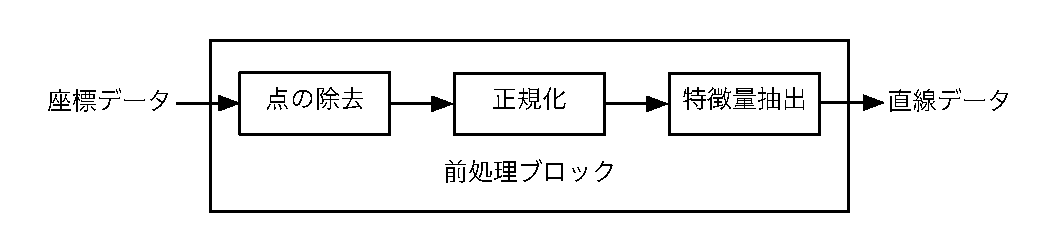
\includegraphics{img/preprocess.eps}}
  \caption{前処理ブロックの概要}
  \label{preprocess}
\end{center}
\end{figure}

\subsubsection{余分な点の除去}
\label{remove_points}
\textbf{図~\ref{extra}(a)}にオリジナルの単語データの例と, \textbf{図~\ref{extra}(b)} に余分な点が除去された後の単語データの例を示す.
収集する医療用語手書きデータは,\textbf{図~\ref{original}}で示したように$(x, y)$座標の時系列データとして存在している.本論文では文献\cite{zhang18:drawing}に従って,これに各点の筆順情報$s$を合わせた$(x, y, s)$を収集する.1つの単語を式~\ref{dataSt}のように収集する.
\begin{equation}
 [[x_1, y_1, s_1], [x_2, y_2, s_2],..., [x_n, y_n, s_n]]
 \label{dataSt}
\end{equation}
$x_i$と$y_i$は点の座標,$s_i$はその点が何画目のストローク上にあるかを示したものである.

手書きデータは書くスピードの違いなどが原因で,同じ単語でもデータ提供者によって点の数が大きく異なってしまい,うまく認識ができない可能性がある.本論文では先行研究に従い,取り除いても文字として成り立つような点の除去を行うことでデータ提供者ごとの点の数の差を小さくする.

\begin{figure}[tb]
 \centering
  \begin{tabular}{c}
   \begin{minipage}[b]{0.5\hsize}
    \centering
    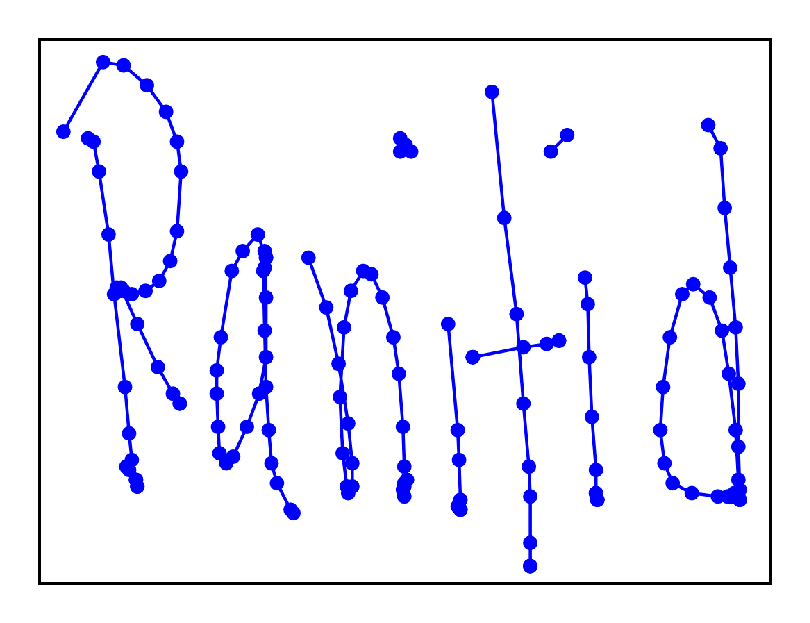
\includegraphics[keepaspectratio,scale=0.5]{img/ranitid.eps}\\
    (a)オリジナルデータ
   \end{minipage}\\
    % \hfill
   \begin{minipage}[b]{0.5\hsize}
    \centering
    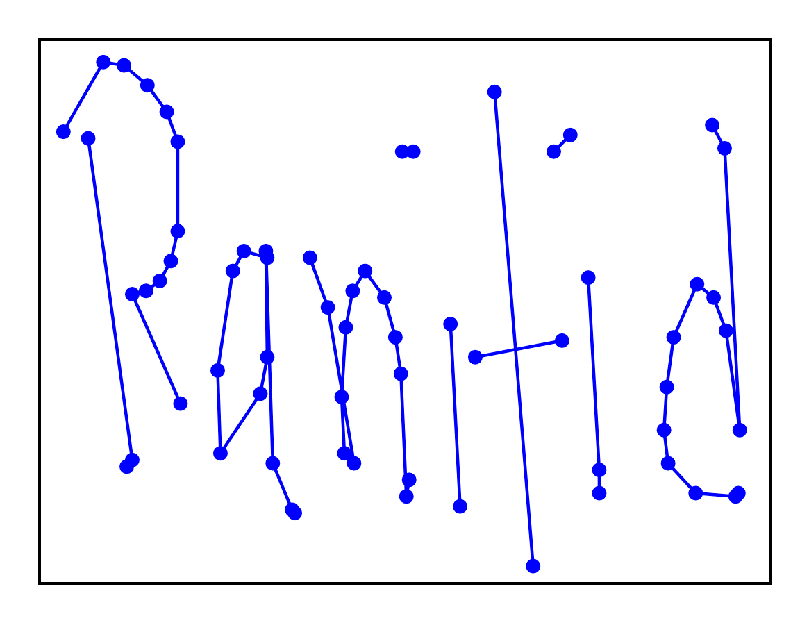
\includegraphics[keepaspectratio,scale=0.5]{img/ranitidClose.eps}\\
    (b)点の除去後
   \end{minipage}
  \end{tabular}
 \caption{データ前処理:余分な点の除去}
 \label{extra}
\end{figure}

\subsubsection{正規化}
\label{normal}
入力データをさらに簡潔にするため,点の除去を施したデータの正規化を行う.はじめに$x$座標についての正規化の手順を説明する.全てのデータの中から最大値$x_{max}$と最小値$x_{min}$を取り出し,式~\ref{eq:normalize}を用いてある点の$x$座標$X$を$X_{nor}$に正規化する.

\begin{equation}
  X_{nor} = \frac{X - x_{min}}{x_{max}-x_{min}}
  \label{eq:normalize}
\end{equation}
$y$座標に対しても同様の計算を行い,結果的に$(x, y)$をそれぞれ$0$以上$1$以下のデータとする.

\subsection{特徴量抽出}
\label{extract}
機械学習への入力のため,特徴量を抽出する.正規化した点データ2点間を繋ぎ,直線データを作成する.直線データに変換することで,点の座標だけでなく直線の長さ,角度などより多くの特徴量を抽出することができる.線データ$L_i$は,点$i$と点$i+1$から式~\ref{eq:line}のように構成され,本論文ではこのデータを学習における入力データとする.

\begin{equation}
  L_i = [x_i, y_i, \Delta{x_i}, \Delta{y_i}, I(s_i=s_{i+1}), I(s_i \neq s_{i+1})]
  \label{eq:line}
\end{equation}
ここで,$\Delta{x_i}=x_{i+1}-x_i$,$\Delta{y_i}=y_{i+1}-y_i$であり,$I()$は括弧内の条件が真であるときに$1$でありそれ以外では$0$である.$L_i$において$x_i$と$y_i$は直線の始点を表し,$\Delta{x_i}$と$\Delta{y_i}$は線の始点から終点までの$x$軸方向,$y$軸方向の距離を表す.また$I(s_i=s_{i+1})=1$は,直線の始点と終点が同一ストローク上にあることを示し,$I(s_i \neq s_{i+1})=1$はその直線で次のストロークに移ったことを示す.

%========================================================================
\subsection{データ拡張ブロック}
\label{augment}
ここでは様々な手書き文字に対応するためのデータ拡張について説明する.本研究では多様な提供者から大量のデータを得る必要があるが,十分なデータ量を確保するためには非常に多くの労力と時間を要する.そのため複数のデータ拡張手法を適用することで機械学習の際の手書き文字データの多様性を高める.

ここでは,先行研究\cite{takahashi}のデータ拡張手法であるStroke Rotation and Parallel-shift(SRP)手法について説明する.
SRP手法とは,ストロークの回転と平行移動によってデータ量を水増しする手法である.
\subsubsection{ストロークの回転}
ストロークの始点と終点の座標から中点を求め,その点を中心にストローク上の点をそれぞれ回転させることでストローク全体を回転させる.この処理を1つのデータに対して複数回施すことで,データ拡張を行う.

\textbf{図~\ref{rotate}(a)}にストロークの回転の原理を示す.ストロークの始点を$(x_f, y_f)$,終点を$(x_l, y_l)$とする.始点と終点の中点を$(a, b)$とすると,式~\ref{eq:center}より$(a, b)$の値が求められる.

\begin{equation}
  (a, b) = (\frac{x_f+x_l}{2}, \frac{y_f+y_l}{2})
  \label{eq:center}
\end{equation}
ストローク上の任意の点の座標を$(x, y)$としたとき,その点を,点$(a, b)$を中心に角$\theta$だけ移動させた後の座標$(X, Y)$は 式~\ref{eq:rotate}で表される.
\begin{equation}
  \left(
    \begin{array}{r}
        X-a \\
        Y-b
    \end{array}
    \right)
 = \left(
  \begin{array}{rr}
      cos\theta & -sin\theta \\
      sin\theta & cos\theta
  \end{array}
  \right)
  \left(
    \begin{array}{r}
        x-a \\
        y-b
    \end{array}
    \right)
  \label{eq:rotate}
\end{equation}
この式をストローク上のすべての点に用いることで,ストローク自体を角$\theta$回転させる.\textbf{図~\ref{rotate}(b)}にストローク回転前の単語データの例,\textbf{図~\ref{rotate}(c)}にストローク回転後の単語データの例を示す.この処理を,ストロークごとに角度を変えながら行うことで元のデータとは異なる形の文字・単語を生成する.それを1つの単語データに対して$N$回行い,データ量を$N$倍に拡張する.

\begin{figure}[tb]
 \centering
  \begin{tabular}{c}
   \begin{minipage}[b]{0.7\hsize}
    \centering
    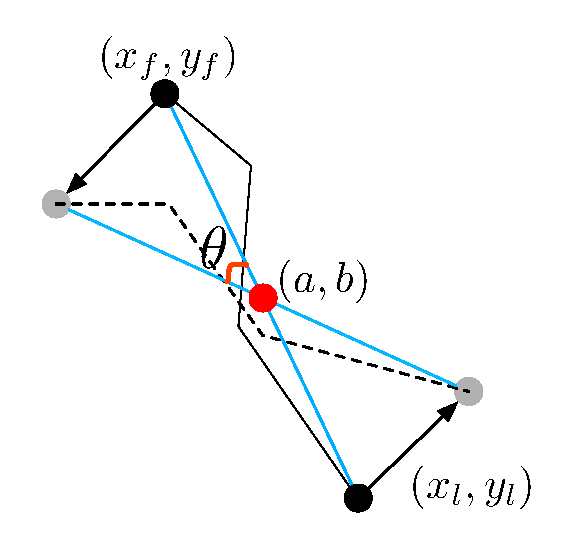
\includegraphics[keepaspectratio,scale=0.7]{img/rotate.eps}\\
    (a)回転の原理
   \end{minipage}\\
    \hfill
   \begin{minipage}[b]{0.5\hsize}
    \centering
    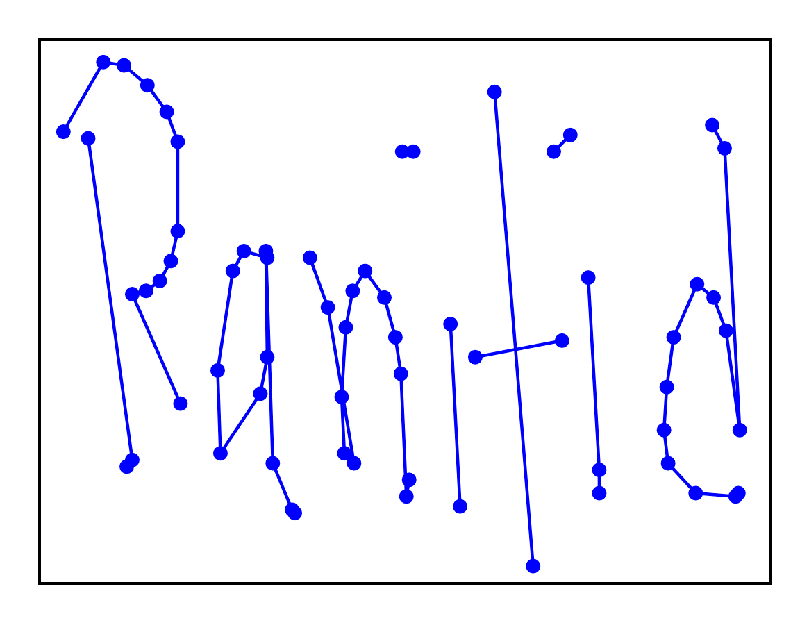
\includegraphics[keepaspectratio,scale=0.5]{img/ranitidCloseBlue.eps}\\
    (b)データ前処理後
   \end{minipage}
   \begin{minipage}[b]{0.5\hsize}
    \centering
    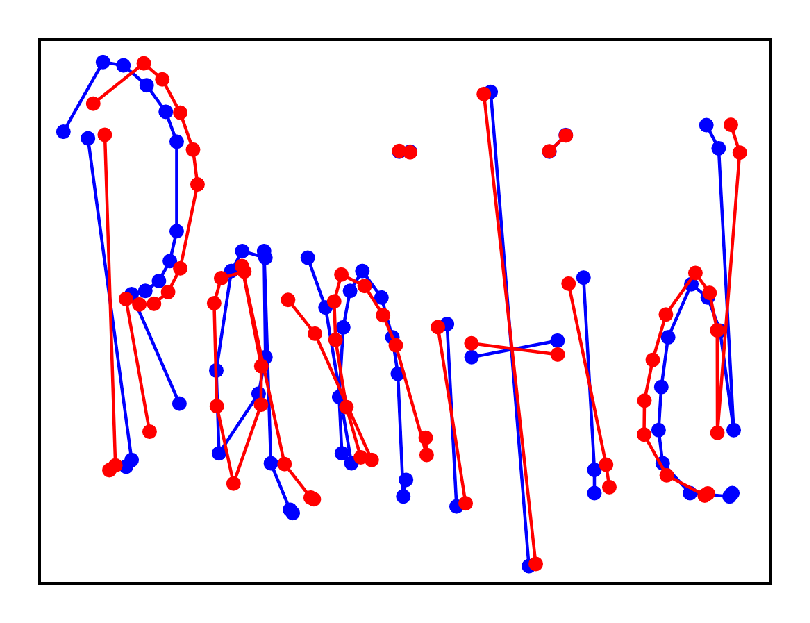
\includegraphics[keepaspectratio,scale=0.5]{img/ranitidRotateRedBlue.eps}\\
    (c)回転前(青)と回転後(赤)
   \end{minipage}
  \end{tabular}
 \caption{ストロークの回転}
 \label{rotate}
\end{figure}

\subsubsection{ストロークの平行移動}
ストローク上の点の座標それぞれに一定の値を加え,ストローク全体を平行移動させることでデータ拡張を行う.\textbf{図~\ref{parallel}(a)}にストロークの平行移動の原理を示す.ストローク上の任意の点の座標を$(x, y)$としたとき,その点を$x$方向に$dx$,$y$方向に$dy$だけ平行移動させた後の座標$(X, Y)$は 式~\ref{eq:parallel}で表される.

\begin{equation}
  (X, Y) = (x+dx, y+dy)
  \label{eq:parallel}
\end{equation}
この式をストローク上のすべての点に用いることで,ストローク自体を$x$方向に$dx$,$y$方向に$dy$平行移動させる.\textbf{図~\ref{parallel}(b)}にストローク平行移動前の単語データの例,\textbf{図~\ref{parallel}(c)}にストローク平行移動後の単語データの例を示す.この処理を,ストロークごとに$dx$と$dy$の値を変えながら行うことで元のデータとは異なる形の文字・単語を生成する.それを1つの単語データに対して$N$回行い,データ量を$N$倍に拡張する.

\begin{figure}[tb]
 \centering
  \begin{tabular}{c}
   \begin{minipage}[b]{0.7\hsize}
    \centering
    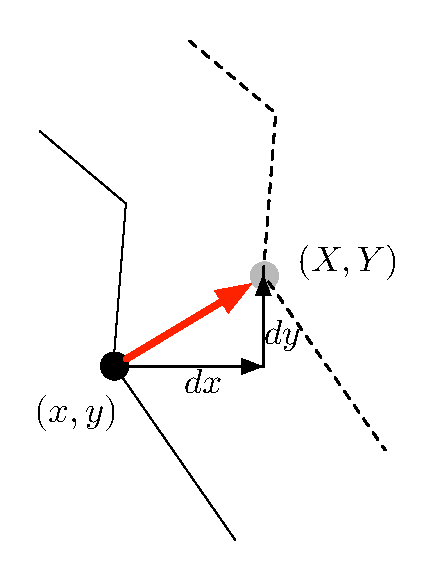
\includegraphics[keepaspectratio,scale=0.7]{img/parallel.eps}\\
    (a)平行移動の原理
   \end{minipage}\\
    \hfill
   \begin{minipage}[b]{0.5\hsize}
    \centering
    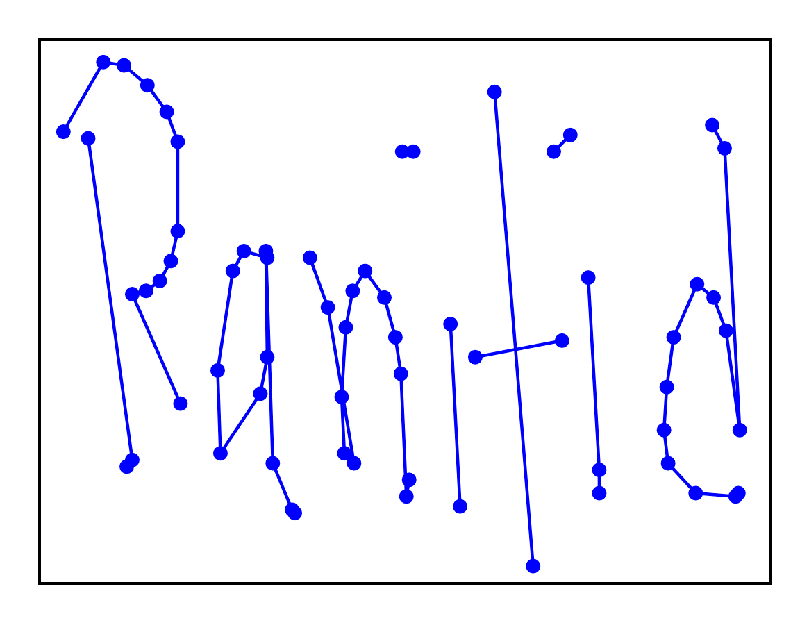
\includegraphics[keepaspectratio,scale=0.5]{img/ranitidCloseBlue.eps}\\
    (b)データ前処理後
   \end{minipage}
   \begin{minipage}[b]{0.5\hsize}
    \centering
    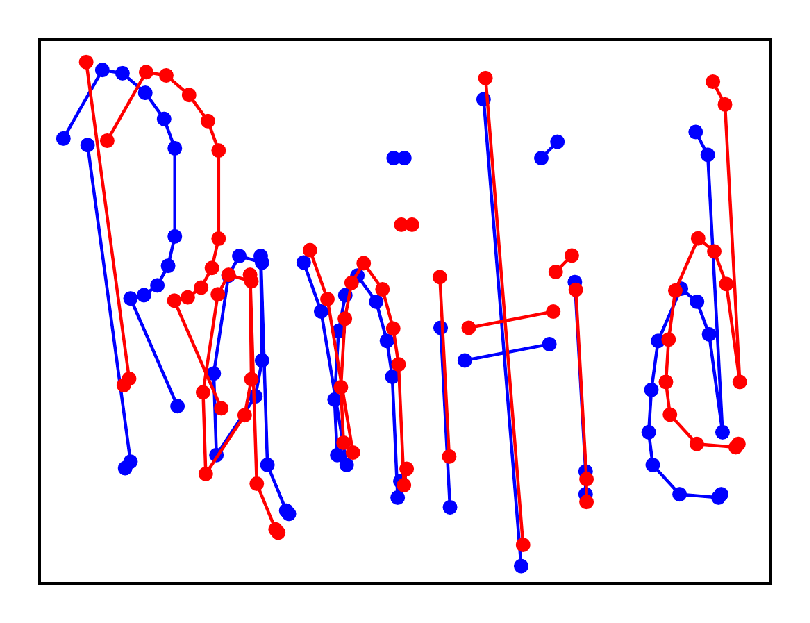
\includegraphics[keepaspectratio,scale=0.5]{img/ranitidParallelRedBlue.eps}\\
    (c)平行移動前(青)と平行移動後(赤)
   \end{minipage}
  \end{tabular}
 \caption{ストロークの平行移動}
 \label{parallel}
\end{figure}

\subsection{機械学習ブロック}
\label{sec:m_learning}
本論文ではBidirectionalLSTMを用いて学習を行う.\textbf{図~\ref{blstm}}にBidirectionalLSTMの概要を示す.BidirectionalLSTMは従来のLSTMに未来の入力から計算を行う逆方向のモデルを加え,出力を同一の出力層に統合するものである.学習プロセスでは,データ拡張が施された直線データを入力として用いる.本論文においてBidirectionalLSTMは,現在入力されている直線データより前に書かれた直線データだけでなく,後に書かれる直線データも用いて学習を行う.推定プロセスでは,学習が行われたモデルに前処理後のデータを入力し,用語の推定を行う.

学習モデルは先行研究を参考に作成し,実装にはpythonのニューラルネットワークライブラリであるKeras\cite{keras}を用いている.活性化関数にはSoftmax関数\cite{softmax}を用いて出力を確率として解釈し,最も確率の高い項目を予測値として決定している.損失関数にはcategorical\_crossentropy\cite{categoricalcrossentropy},最適化関数にはAdam\cite{kingma14:adam}を用いており,学習の評価は正解率で計算を行なっている.

\begin{figure}[tb]
 \begin{center}
  \resizebox{\columnwidth}{!}{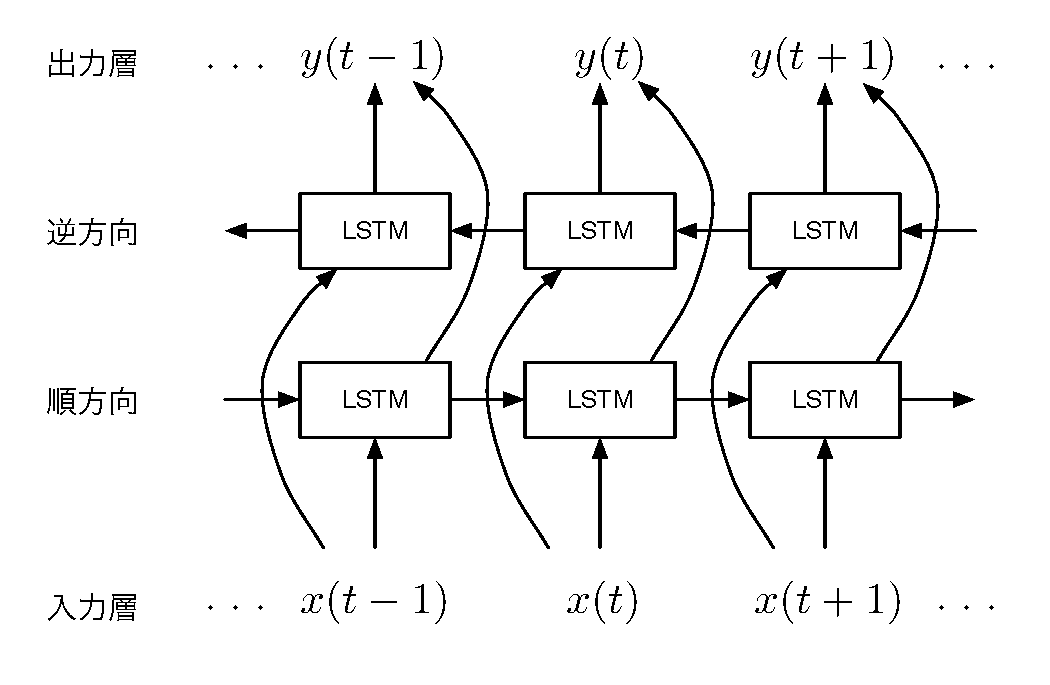
\includegraphics{img/blstm.eps}}
  \caption{BidirectionalLSTMの概要}
  \label{blstm}
\end{center}
\end{figure}


% 以下はRefTeX用
%%% Local Variables:
%%% mode: yatex
%%% TeX-master: "thesis"
%%% End:
